

% RECOMMENDED %%%%%%%%%%%%%%%%%%%%%%%%%%%%%%%%%%%%%%%%%%%%%%%%%%%
\documentclass[graybox]{svmult}

% choose options for [] as required from the list
% in the Reference Guide

%\usepackage{type1cm}        % activate if the above 3 fonts are
%                            % not available on your system
%
%\usepackage{makeidx}         % allows index generation
\usepackage{graphicx}        % standard LaTeX graphics tool
                             % when including figure files
\usepackage{multicol}        % used for the two-column index
\usepackage[bottom]{footmisc}% places footnotes at page bottom
\usepackage{framed} % vince may 17


\usepackage{newtxtext}       % 
\usepackage[varvw]{newtxmath}       % selects Times Roman as basic font

% see the list of further useful packages
% in the Reference Guide

%\makeindex             % used for the subject index
                       % please use the style svind.ist with
                       % your makeindex program

%%%%%%%%%%%%%%%%%%%%%%%%%%%%%%%%%%%%%%%%%%%%%%%%%%%%%%%%%%%%%%%%%%%%%%%%%%%%%%%%%%%%%%%%%

\begin{document}

\title*{Bioconductor's Computational Ecosystem for Genomic Data Science in Cancer}
\titlerunning{Bioconductor for Cancer Data Science}
% Use \titlerunning{Short Title} for an abbreviated version of
% your contribution title if the original one is too long
\author{Name of First Author\orcidID{0000-1111-2222-3333} and\\ Name of Second Author\orcidID{1111-2222-3333-4444}}
% Use \authorrunning{Short Title} for an abbreviated version of
% your contribution title if the original one is too long
\institute{Name of First Author \at Name, Address of Institute, \email{name@email.address}
\and Name of Second Author \at Name, Address of Institute \email{name@email.address}}
%
% Use the package "url.sty" to avoid
% problems with special characters
% used in your e-mail or web address
%
\maketitle

\abstract{
The Bioconductor project enters its third decade with over two 
thousand packages for genomic data science, over 100,000 annotation and 
experiment resources, and a global system for convenient distribution to 
researchers. Over 60,000 PubMed Central citations and terabytes of content 
shipped per month attest to the impact of the project 
on cancer genomic data science. This report provides an overview 
of cancer genomics resources in Bioconductor. After an overview 
of Bioconductor project principles, we address exploration 
of institutionally curated cancer genomics data such as TCGA. 
We then review genomic annotation and ontology resources 
relevant to cancer and then briefly survey analytical 
workflows addressing specific topics in cancer genomics. 
Concluding sections cover how new software and data 
resources are brought into the ecosystem and how the 
project is tackling needs for training of the research 
workforce. Bioconductor's strategies for supporting 
methods developers and researchers in cancer genomics 
are evolving along with experimental and computational 
technologies. All the tools described in this report 
are backed by regularly maintained learning resources 
that can be used locally or in cloud computing environments.
}



\section{Introduction}
\label{sec:1}

Computation is a central component of cancer genomics
research. Tumor sequencing is the basis of computational
investigation of mutational, epigenetic and immunologic
processes associated with cancer initiation and progression.
Numerous computational workflows have been produced to
profile tumor cell transcriptomes and proteomes.
New technologies promise to unite sequence-based
characterizations with digital histopathology,
ultimately driving efforts in molecule design
and evaluation to produce patient-centered treatments.

Bioconductor is an open source software project with
a 20 year history of uniting biostatisticians, bioinformaticians,
and genome researchers in the creation of an ecosystem
of data, annotation, and analysis resources for research
in genome-scale biology. This paper will review current
approaches of the project to advancing cancer genomics.
After a brief discussion of basic principles of the Bioconductor
project, we will present a ``top down'' survey of resources
useful for cancer bioinformatics. Primary sections address

\begin{itemize}
\tightlist
\item
  how to explore institutionally curated cancer genomics data
\item
  genomic annotation resources relevant to cancer genomics
\item
  analytical workflows
\item
  components for introducing new data or analyses
\item
  pedagogics and workforce development.
\end{itemize}

\section{Bioconductor principles}


\subsection{R packages and vignettes}\label{r-packages-and-vignettes}}

Software tools and data resources in Bioconductor are organized
into ``R packages''. These are collections of folders with data,
code (principally R functions), and documentation
following a protocol specified in
\href{https://cran.r-project.org/doc/manuals/R-exts.html}{Writing R Extensions}. R packages have a DESCRIPTION file with metadata about
package contents and provenance. Package structure can be
checked for validity using the \texttt{R CMD check} facility.
Documentation of code and data can be programmatically
checked for existence and validity. The DESCRIPTION file
for a package specifies its version and
also gives precise definition of how an R package may
depend upon versions of other packages.

At its inception,
Bioconductor introduced a new approach to holistic package
documentation called ``vignette''.
Vignettes provide narrative and explanation interleaved with
executable code describing package operations.
While R function manual pages describe
the operation of individual functions,
vignettes illustrate the interoperation
of package components and provide motivation
for both package design but also context
for its use.

\subsection{R package repositories; repository evolution}\label{r-package-repositories-repository-evolution}}

Bioconductor software forms a coherent ecosystem that
can be checked for consistency of versions of all
packages available in a given installation of R.
Bioconductor packages may specify dependency on
other Bioconductor packages, or packages that are
available in the CRAN repository. Bioconductor does
not include packages with dependencies on ``github-only''
packages. Later in this paper we will provide details
on package quality assurance that provide a rationale
for this restriction.

Major updates to the R language occur annually, and
updates are preceded by careful assessment of effects of
language change on Bioconductor package operations. These effects
can be identified through changes in the output of R CMD check.
The Bioconductor ecosystem is updated twice a year, once
to coincide with update to R, and once about six months
later. The semianual updates reflect the need to track
developments in the fast-moving field of genomic data science.

\subsection{Package quality assessment; installation consistency}\label{package-quality-assessment-installation-consistency}}

The BiocCheck function is used to provide more
stringent assessment of package compliance with basic
principles of the Bioconductor ecosystem.

The BiocManager package provides for installing and updating package
and has functionality for verifying the coherence and version status
of the currently installed package collection.
This is important
in the context of a language and package ecosystem
that changes every six months, while analyses may
take years to complete. Tools for recreating past
package collections are available to assist in
reproducing outputs of prior analyses.

\subsection{Unifying assay and sample data: SummarizedExperiment and MultiAssayExperiment}\label{unifying-assay-and-sample-data-summarizedexperiment-and-multiassayexperiment}}

Most of the data from genome-scale experiments to be discussed
in this chapter are organized in special data containers
rooted in the concepts of the SummarizedExperiment class.
Briefly, assay data are thought of as occupying a \(G \times N\)
array, and sample level data occupy an \(N \times K\) table. The array
and the table are linked together in the SummarizedExperiment; see Figure \ref{fig:sesc}.

\begin{figure}
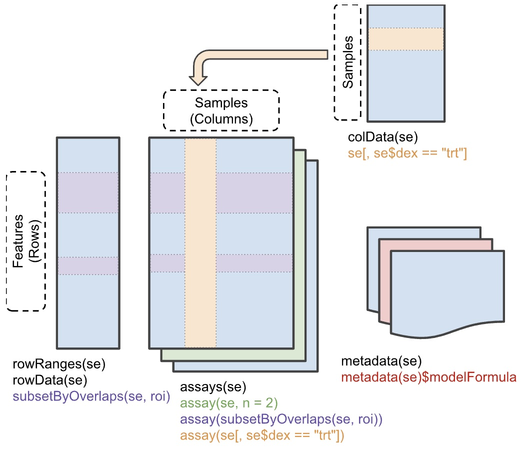
\includegraphics[width=0.8\linewidth,]{SEschema} \caption{SummarizedExperiment schematic.}\label{fig:sesc}
\end{figure}

Multiple representations of assay results may be managed in this
structure, but all assay arrays must have dimensions \(G \times N\).

For experiment collections in which the same samples are subjected
to multiple genome-scale assays, MultiAssayExperiment containers are used. See Figure \ref{fig:masc} for the layout.

\begin{figure}
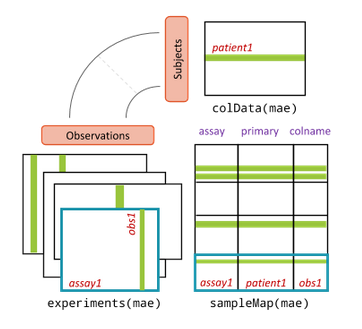
\includegraphics[width=0.8\linewidth,]{MAEschema} \caption{MultiAssayExperiment schematic.}\label{fig:masc}
\end{figure}

Further details on these data structures will be provided in section \ref{class}.

\subsection{Downloading and caching cancer genomics data and annotations}\label{cache}}

Downloading and managing data from various online resources
can be excessively time consuming. Bioconductor encourages data caching for
increased efficiency and reproducibility. The caching data methods
employed in Bioconductor
allow analysis code to
concisely refer to data resources as needed, with minimal attention to how
data are stored, retrieved or transformed.
It allows for easy management and reuse of data that are on remote
servers or in cloud, storing source
location and providing information for data updates. The BiocFileCache
Bioconductor package handles data management from within R.

BiocFileCache is a general-use caching system but Bioconductor also provides
``Hubs'', AnnotationHub and ExperimentHub, to help distributed annotation or
experimental data hosted externally. Both AnnotationHub and ExperimentHub use
BiocFileCache to handle download and caching of data.

AnnotationHub provides a centralized repository of diverse genomic annotations,
facilitating easy access and integration into analyses. Researchers can
seamlessly retrieve information such as genomic features, functional
annotations, and variant data, streamlining the annotation process for their
analyses.

ExperimentHub extends this concept to experimental data. It serves as a
centralized hub for storing and sharing curated experiment-level datasets,
allowing researchers to access a wide range of experimental designs and
conditions. This cloud-based infrastructure enhances collaboration and promotes
the reproducibility of analyses across different laboratories.

The curatedTCGAData package provides some resources through
ExperimentHub, as do many other self-identified ``CancerData'' resources. Once the
ExperimentHub is loaded, it can be queried for terms of interest.

\begin{shaded}
\begin{verbatim}
library(ExperimentHub)
eh = ExperimentHub()
query(eh, "CancerData")
\end{verbatim}
\end{shaded}

%\texttt{\{r useeh\} \textless{}!-\/- , fig.cap="ExperimentHub attachment, retrieval, query, and response when seeking cancer-related data.", message=FALSE\} -\/-\textgreater{} library(ExperimentHub) eh \textless{}- ExperimentHub() query(eh, "CancerData")}

Multiple terms can be used to narrow results before choosing a download.

\begin{shaded}
\begin{verbatim}
query(eh, c("CancerData", "esophageal"))
# ExperimentHub with 2 records}
# snapshotDate(): 2023-10-24}
# $dataprovider: University of California San Francisco}
# $species: Homo sapiens}
# $rdataclass: RangedSummarizedExperiment, data.frame}
# additional mcols(): taxonomyid, genome, description,}
#   coordinate_1_based, maintainer, rdatadateadded, preparerclass, tags,}
#   rdatapath, sourceurl, sourcetype }
# retrieve records with, e.g., object[["EH8527"]]
#            title                           
#   EH8527 | cao_esophageal_wgbs_hg19        
#   EH8530 | cao_esophageal_transcript_counts
\end{verbatim}
\end{shaded}

Similarly AnnotationHub files can be downloaded for annotating data. For example,
the ensembl 110 release of gene and protein annotations are obtained with the
following:

\begin{shaded}
\begin{verbatim}
library(AnnotationHub)
ah = AnnotationHub()
query(ah, c("ensembl", "110"))
\end{verbatim}
\end{shaded}


\section{Exploring institutionally curated cancer genomics data}\label{exploring-institutionally-curated-cancer-genomics-data}}


\subsection{The Cancer Genome Atlas}\label{the-cancer-genome-atlas}}

An overview of Bioconductor's resource for the Cancer
Genome Atlas (TCGA) is easy to obtain, with the
curatedTCGAData package.

\begin{shaded}
\begin{verbatim}
library(curatedTCGAData)
tcgatab = curatedTCGAData(version="2.1.1")
\end{verbatim}
\end{shaded}
%\begin{Shaded}
%\begin{Highlighting}[]
%\KeywordTok{library}\NormalTok{(curatedTCGAData)}
%\NormalTok{tcgatab =}\StringTok{ }\KeywordTok{curatedTCGAData}\NormalTok{(}\DataTypeTok{version=}\StringTok{"2.1.1"}\NormalTok{)}
%\end{Highlighting}
%\end{Shaded}

Records obtained for adrenocortical carcinoma (code ACC) are in Table \ref{tab:tab-lktab}.

\begin{table}

\caption{\label{tab:tab-lktab}Records returned by curatedTCGAData::curatedTCGAData(), filtered to those pertaining to adrenocortical carcinoma.}
\centering
\begin{tabular}[t]{lllll}
\toprule
  & ah\_id & title & file\_size & rdataclass\\
\midrule
1 & EH4737 & ACC\_CNASNP-20160128 & 0.8 Mb & RaggedExperiment\\
2 & EH4738 & ACC\_CNVSNP-20160128 & 0.2 Mb & RaggedExperiment\\
3 & EH4740 & ACC\_GISTIC\_AllByGene-20160128 & 0.2 Mb & SummarizedExperiment\\
4 & EH4741 & ACC\_GISTIC\_Peaks-20160128 & 0 Mb & RangedSummarizedExperiment\\
5 & EH4742 & ACC\_GISTIC\_ThresholdedByGene-20160128 & 0.2 Mb & SummarizedExperiment\\
\addlinespace
6 & EH4744 & ACC\_Methylation-20160128\_assays & 239.2 Mb & SummarizedExperiment\\
7 & EH4745 & ACC\_Methylation-20160128\_se & 6 Mb & RaggedExperiment\\
8 & EH4747 & ACC\_Mutation-20160128 & 0.7 Mb & SummarizedExperiment\\
9 & EH4748 & ACC\_RNASeq2Gene-20160128 & 2.7 Mb & SummarizedExperiment\\
10 & EH4750 & ACC\_RPPAArray-20160128 & 0.1 Mb & SummarizedExperiment\\
\addlinespace
414 & EH8118 & ACC\_miRNASeqGene-20160128 & 0.2 Mb & SummarizedExperiment\\
415 & EH8119 & ACC\_RNASeq2GeneNorm-20160128 & 5.4 Mb & SummarizedExperiment\\
\bottomrule
\end{tabular}
\end{table}

Various conventions are in play in this table. The ``title'' field is
of primary concern. The title string can be decomposed into
substrings with interpretation
\texttt{{[}tumorcode{]}\_{[}assay{]}-{[}date{]}\_{[}optional codes{]}}. The column \texttt{ah\_id} will be
explained in section \ref{hubs}, and entries in column
\texttt{rdataclass} will be discussed in section \ref{class} below.


\subsubsection{Tumor code resolution}\label{tumor-code-resolution}}

There are 33 different tumor types available in TCGA. The
decoding of tumor codes for the first ten in alphabetical order is
provided in Table \ref{tab:tab-deco}.

\begin{table}

\caption{\label{tab:tab-deco}Decoding TCGA tumor code abbreviations.}
\centering
\begin{tabular}[t]{ll}
\toprule
Code & Tumor.Type\\
\midrule
ACC & Adrenocortical Carcinoma\\
BLCA & Bladder Urothelial Carcinoma\\
BRCA & Breast Invasive Carcinoma\\
CESC & Cervical Squamous Cell Carcinoma and Endocervical Adenocarcinoma\\
CHOL & Cholangiocarcinoma\\
\addlinespace
CNTL & Controls\\
COAD & Colon Adenocarcinoma\\
DLBC & Lymphoid Neoplasm Diffuse Large B-cell Lymphoma\\
ESCA & Esophageal Carcinoma\\
FPPP & FFPE Pilot Phase II\\
\addlinespace
GBM & Glioblastoma Multiforme\\
HNSC & Head and Neck Squamous Cell Carcinoma\\
KICH & Kidney Chromophobe\\
KIRC & Kidney Renal Clear Cell Carcinoma\\
KIRP & Kidney Renal Papillary Cell Carcinoma\\
\addlinespace
LAML & Acute Myeloid Leukemia\\
LCML & Chronic Myelogenous Leukemia\\
LGG & Brain Lower Grade Glioma\\
LIHC & Liver Hepatocellular Carcinoma\\
LUAD & Lung Adenocarcinoma\\
\addlinespace
LUSC & Lung Squamous Cell Carcinoma\\
MESO & Mesothelioma\\
MISC & Miscellaneous\\
OV & Ovarian Serous Cystadenocarcinoma\\
PAAD & Pancreatic Adenocarcinoma\\
\addlinespace
PCPG & Pheochromocytoma and Paraganglioma\\
PRAD & Prostate Adenocarcinoma\\
READ & Rectum Adenocarcinoma\\
SARC & Sarcoma\\
SKCM & Skin Cutaneous Melanoma\\
\addlinespace
STAD & Stomach Adenocarcinoma\\
TGCT & Testicular Germ Cell Tumors\\
THCA & Thyroid Carcinoma\\
THYM & Thymoma\\
UCEC & Uterine Corpus Endometrial Carcinoma\\
\addlinespace
UCS & Uterine Carcinosarcoma\\
UVM & Uveal Melanoma\\
\bottomrule
\end{tabular}
\end{table}


\subsubsection{Assay codes and counts}\label{assay-codes-and-counts}}

Assays performed on tumors vary across tumor types. For assay
types shared between
breast cancer, glioblastoma, and lung adenocarcinoma (code LUAD),
the numbers of tumor and normal samples available in curatedTCGAData
are provided in Table \ref{tab:tab-doassc}.

\begin{table}

\caption{\label{tab:tab-doassc}Numbers of assays available in TCGA on tumor and normal samples,
for breast cancer, glioblastoma, and lung adenocarcinoma.}
\centering
\begin{tabular}[t]{lrrrrrr}
\toprule
  & BRCA & BRCAnormal & GBM & GBMnormal & LUAD & LUADnormal\\
\midrule
CNASNP & 1089 & 1120 & 577 & 527 & 516 & 579\\
CNVSNP & 1080 & 1119 & 577 & 527 & 516 & 579\\
GISTIC\_AllByGene & 1080 & 0 & 577 & 0 & 516 & 0\\
GISTIC\_Peaks & 1080 & 0 & 577 & 0 & 516 & 0\\
GISTIC\_ThresholdedByGene & 1080 & 0 & 577 & 0 & 516 & 0\\
\addlinespace
Mutation & 988 & 5 & 283 & 7 & 230 & 0\\
RNASeq2Gene & 1093 & 119 & 153 & 13 & 515 & 61\\
RPPAArray & 887 & 50 & 233 & 11 & 365 & 0\\
RNASeq2GeneNorm & 1093 & 119 & 153 & 13 & 515 & 61\\
Methylation\_methyl27 & 314 & 29 & 285 & 0 & 65 & 24\\
\addlinespace
Methylation\_methyl450 & 783 & 102 & 140 & 14 & 458 & 34\\
\bottomrule
\end{tabular}
\end{table}


\subsubsection{An example dataset for RNA-seq from glioblastoma multiforme}\label{an-example-dataset-for-rna-seq-from-glioblastoma-multiforme}}

We obtain normalized RNA-seq data on primary tumor samples for GBM with

%\begin{Shaded}
%\begin{Highlighting}[]
%\NormalTok{gbrna =}\StringTok{ }\KeywordTok{TCGAprimaryTumors}\NormalTok{(}\KeywordTok{curatedTCGAData}\NormalTok{(}\StringTok{"GBM"}\NormalTok{, }
%    \StringTok{"RNASeq2GeneNorm"}\NormalTok{, }\DataTypeTok{dry.run=}\OtherTok{FALSE}\NormalTok{, }\DataTypeTok{version=}\StringTok{"2.1.1"}\NormalTok{))}
%\NormalTok{gbrna}
%\CommentTok{\#\# A MultiAssayExperiment object of 1 listed}
%\CommentTok{\#\#  experiment with a user{-}defined name and respective class.}
%\CommentTok{\#\#  Containing an ExperimentList class object of length 1:}
%\CommentTok{\#\#  [1] GBM\_RNASeq2GeneNorm{-}20160128: SummarizedExperiment with 18199 rows and 153 columns}
%\CommentTok{\#\# Functionality:}
%\CommentTok{\#\#  experiments() {-} obtain the ExperimentList instance}
%\CommentTok{\#\#  colData() {-} the primary/phenotype DataFrame}
%\CommentTok{\#\#  sampleMap() {-} the sample coordination DataFrame}
%\CommentTok{\#\#  \textasciigrave{}$\textasciigrave{}, \textasciigrave{}[\textasciigrave{}, \textasciigrave{}[[\textasciigrave{} {-} extract colData columns, subset, or experiment}
%\CommentTok{\#\#  *Format() {-} convert into a long or wide DataFrame}
%\CommentTok{\#\#  assays() {-} convert ExperimentList to a SimpleList of matrices}
%\CommentTok{\#\#  exportClass() {-} save data to flat files}
%\end{Highlighting}
%\end{Shaded}

\begin{shaded}
\begin{verbatim}
gbrna = TCGAprimaryTumors(curatedTCGAData("GBM",
     "RNASeq2GeneNorm", dry.run=FALSE, version="2.1.1"))
gbrna
## A MultiAssayExperiment object of 1 listed
##experiment with a user-defined name and respective class.
##Containing an ExperimentList class object of length 1:
[1] GBM_RNASeq2GeneNorm-20160128: SummarizedExperiment with 
##        18199 rows and 153 columns
##
## Functionality:
##experiments() - obtain the ExperimentList instance
##colData() - the primary/phenotype DataFrame
##sampleMap() - the sample coordination DataFrame
##`$`, `[`, `[[` - extract colData columns, subset, or experiment
####*Format() - convert into a long or wide DataFrame
assays() - convert ExperimentList to a SimpleList of matrices
##exportClass() - save data to flat files
\end{verbatim}
\end{shaded}

R functions defined in Bioconductor packages can operate on the variable \texttt{gbrna} to
retrieve information of interest. Details on the underlying data structure
are given in section \ref{class} below. For most assay types, we think of the quantitative
assay
information as tabular in nature, with table rows corresponding to genomic
features such as genes, and table columns corresponding to samples.

Information on GBM samples employs the \texttt{colData} function.

%\begin{shaded}
%\begin{Highlighting}[]
%\KeywordTok{dim}\NormalTok{(}\KeywordTok{colData}\NormalTok{(gbrna))}
%\CommentTok{\#\# [1]  153 4380}
%\end{Highlighting}
%\end{shaded}


\begin{shaded}
\begin{verbatim}
dim(colData(gbrna))
## [1] 153 4380
\end{verbatim}
\end{shaded}

For sample level information obtained \texttt{colData}, we think of rows
as samples, and columns as sample attributes.


\subsubsection{Clinical and phenotypic data}
\label{clinical-and-phenotypic-data}}

TCGA datasets are generally provided as combinations of
results for tumor tissue and normal tissue. The determination
of a record's sample type is encoded in the sample ``barcode''.
Decoding of sample barcodes is described at 

\begin{verbatim}
https://docs.gdc.cancer.gov/Encyclopedia/pages/TCGA_Barcode/
\end{verbatim}

\noindent
with specific interpretation of sample types listed 
at
{\small
\begin{verbatim}
https://gdc.cancer.gov/resources-tcga-users/tcga-code-tables/sample-type-codes
\end{verbatim}
}
\noindent
separately. The TCGAutils package provides utilities for extracting
data on primary tumor samples, excluding samples that may have been taken on
normal tissue or metastases.

Clinical and phenotypic data on all TCGA samples are voluminous. For example,
there are 2684 fields of sample level data for BRCA
samples, and 4380 fields for GBM samples. Many of these
fields are meaningfully populated for only a very small minority of samples.
To see this for GBM:

%\begin{shaded}
%\begin{Highlighting}[]
%\KeywordTok{mean}\NormalTok{(}\KeywordTok{sapply}\NormalTok{(}\KeywordTok{colData}\NormalTok{(gbrna), }\ControlFlowTok{function}\NormalTok{(x) }\KeywordTok{mean}\NormalTok{(}\KeywordTok{is.na}\NormalTok{(x))}\OperatorTok{\textgreater{}}\NormalTok{.}\DecValTok{90}\NormalTok{))}
%\CommentTok{\#\# [1] 0.8091324}
%\end{Highlighting}
%\end{shaded}

\begin{shaded}
\begin{verbatim}
mean(sapply(colData(gbrna), function(x) mean(is.na(x))>.90))
## [1] 0.8091324
\end{verbatim}
\end{shaded}

In words, for 81\% of clinical data fields in TCGA GBM data,
at least 90\% of entries are missing.

Nevertheless, with careful inspection of fields and contents,
nearly complete clinical data can be extracted and combined with molecular
and genetic assay data with modest effort.

The following code chunk illustrates a very crude
approach to comparing survival profiles for BRCA, GBM, and LUAD
donors. The result is in Figure \ref{fig:dothesurv}.


{\small
\begin{shaded}
\begin{verbatim}
# obtain mutation data for BRCA, GBM, LUAD; could use any or all assay types
brmut = curatedTCGAData("BRCA", "Mutation", version = "2.1.1", dry.run = FALSE)
gbmut = curatedTCGAData("GBM", "Mutation", version = "2.1.1", dry.run = FALSE)
lumut = curatedTCGAData("LUAD", "Mutation", version = "2.1.1", dry.run = FALSE)
# extract survival times
library(survival)
getSurv = function(mae) {
 days_on = with(colData(mae), ifelse(is.na(days_to_last_followup),
 days_to_death, days_to_last_followup))
 Surv(days_on, colData(mae)$vital_status)
}
ss = lapply(list(brmut, gbmut, lumut), getSurv)
codes = c("BRCA", "GBM", "LUAD")
type = factor(rep(codes, sapply(ss,length)))
allsurv = do.call(c, ss)
library(GGally)
ggsurv(survfit(allsurv~type))
\end{verbatim}
\end{shaded}
}

\begin{figure}
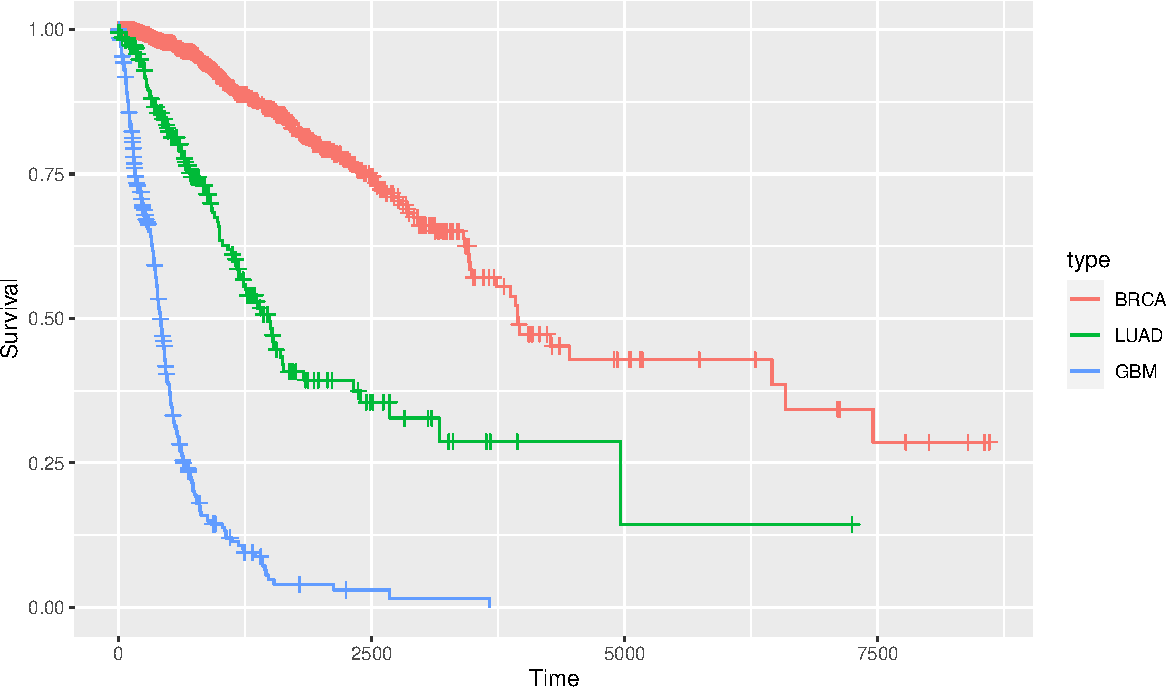
\includegraphics[width=0.8\linewidth,]{bioccb_files/figure-latex/dothesurv-1} \caption{Survival profile extraction from three MultiAssayExperiments produced with curatedTCGAData calls.}\label{fig:dothesurv}
\end{figure}

At this point, survival times within tumor type can be stratified by any
features of the mutation profiles of individual samples.
The ``RaggedExperiment'' class is employed to test each BRCA sample for
presence of any mutation in the gene TTN. See Figure \ref{fig:strat}.

\begin{shaded}
\begin{verbatim}
bprim = TCGAprimaryTumors(brmut)
## harmonizing input:
## removing 5 sampleMap rows with 'colname' not in 
##      colnames of experiments
mutsyms = assay(experiments(bprim)[[1]], "Hugo_Symbol")
cn = rownames(colData(bprim)) # short
cna = colnames(mutsyms) # long
cnas = substr(cna, 1, 12)
hasTTNmut = apply(assay(experiments(TCGAprimaryTumors(brmut))[[1]], 
     "Hugo_Symbol"), 2, function(x) length(which(x=="TTN"))>0)
## harmonizing input:
## removing 5 sampleMap rows with 'colname' not in
##      colnames of experiments
names(hasTTNmut) = cnas
bsurv = getSurv(TCGAprimaryTumors(brmut))
## harmonizing input:
## removing 5 sampleMap rows with 'colname' not in 
##      colnames of experiments
hasTTNmut = hasTTNmut[cn] # match mutation records to surv times
ggsurv(survfit(bsurv~hasTTNmut))
\end{verbatim}
\end{shaded}


\begin{figure}
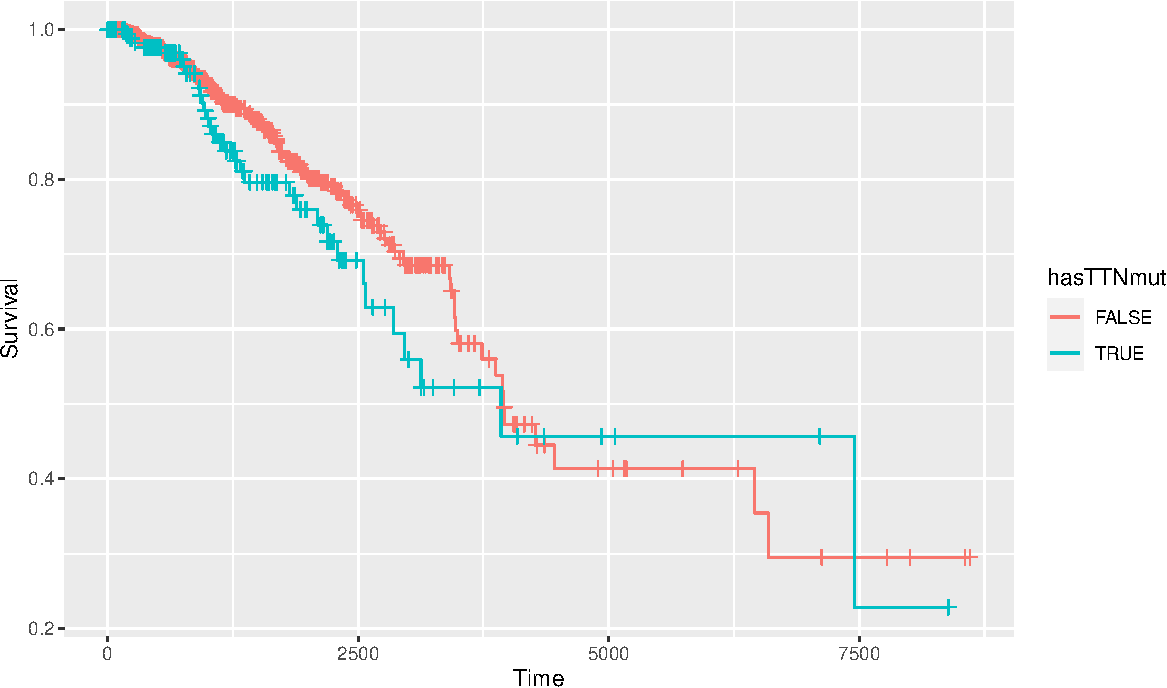
\includegraphics[width=1\linewidth,]{bioccb_files/figure-latex/strat-1} \caption{Survival distributions for donors of breast tumors in TCGA, stratified by presence or absence of mutation in gene TTN.}\label{fig:strat}
\end{figure}

Similar manipulations permit exploration of relationships between
any molecular assay outcomes and any clinical data collected in TCGA.


\subsection{cBioPortal}\label{cbioportal}}

The cBioPortal user guide
at 
\begin{verbatim}
https://www.cbioportal.org/
\end{verbatim}
defines the goal of the portal to be reducing ``the barriers between complex
genomic data and cancer researchers by providing rapid, intuitive, and high-quality
access to molecular profiles and clinical attributes from large-scale cancer genomics projects, and
therefore to empower researchers to translate these rich data sets into biologic insights and clinical applications.''

Bioconductor's cBioPortalData package simplifies access to over 300 genomic studies of
diverse cancers in cBioPortal. The main unit of data access is the publication. The
\texttt{cBioPortal} function mediates a connection between an R session and the
cBioPortal API. \texttt{getStudies} returns a tibble with metadata on
all studies.

\begin{shaded}
\begin{verbatim}
library(cBioPortalData)
cbio = cBioPortal()
allst = getStudies(cbio)
dim(allst)
## [1] 397 13
\end{verbatim}
\end{shaded}

A pruned selection of records from the cBioPortal
studies table is given in Table \ref{tab:tab-cball}.

\begin{table}
\caption{\label{tab:tab-cball}Excerpts from four fields on selected records in the cBioPortal getStudies output.}\\
\begin{tabular}{p{5cm}p{5cm}l}
name & description & studyId \\ \hline
Adenoid Cystic Carcinoma of the Breast & Whole exome sequencing of 12 breast AdCCs. & acbc\_mskcc\_2015 \\
Adenoid Cystic Carcinoma & Whole-exome or whole-genome sequencing analysis of 60 ACC tumor/normal pairs & acyc\_mskcc\_2013 \\
Adenoid Cystic Carcinoma & Targeted Sequencing of 28 metastatic Adenoid Cystic Carcinoma samples. & acyc\_fmi\_2014 \\
Adenoid Cystic Carcinoma & Whole-genome or whole-exome sequencing of 25 adenoid cystic carcinoma tumor/normal pairs. & acyc\_jhu\_2016 \\
Adenoid Cystic Carcinoma & WGS of 21 salivary ACCs and targeted molecular analyses of a validation set (81 patients). & acyc\_mda\_2015 \\
Adenoid Cystic Carcinoma & Whole-genome/exome sequencing of 10 ACC PDX models. & acyc\_mgh\_2016 \\
Adenoid Cystic Carcinoma & Whole exome sequencing of 24 ACCs. & acyc\_sanger\_2013 \\
Adenoid Cystic Carcinoma Project & Multi-Institute Cohort of 1045 Adenoid Cystic Carcinoma patients. & acc\_2019 \\
Basal Cell Carcinoma & Whole-exome sequencing of 126 basal cell carcinoma tumor/normal pairs; targeted sequencing of 163 sporadic samples (40 tumor/normal pairs) and 4 Gorlin symdrome basal cell carcinomas. & bcc\_unige\_2016 \\
\end{tabular}
\end{table}

%\begin{table}[lll]%{>{\raggedright\arraybackslash}p{12em}>{\raggedright\arraybackslash}p{15em}l}
%\caption{\label{tab:tab-cball}Excerpts from four fields on selected records in the cBioPortal getStudies output.}\\
%\toprule
%name & description & studyId\\
%\midrule
%Adenoid Cystic Carcinoma of the Breast & Whole exome sequencing of 12 breast AdCCs. & acbc\_mskcc\_2015\\
%Adenoid Cystic Carcinoma & Whole-exome or whole-genome sequencing analysis of 60 ACC tumor/normal pairs & acyc\_mskcc\_2013\\
%Adenoid Cystic Carcinoma & Targeted Sequencing of 28 metastatic Adenoid Cystic Carcinoma samples. & acyc\_fmi\_2014\\
%Adenoid Cystic Carcinoma & Whole-genome or whole-exome sequencing of 25 adenoid cystic carcinoma tumor/normal pairs. & acyc\_jhu\_2016\\
%Adenoid Cystic Carcinoma & WGS of 21 salivary ACCs and targeted molecular analyses of a validation set (81 patients). & acyc\_mda\_2015\\
%\addlinespace
%Adenoid Cystic Carcinoma & Whole-genome/exome sequencing of 10 ACC PDX models. & acyc\_mgh\_2016\\
%Adenoid Cystic Carcinoma & Whole exome sequencing of 24 ACCs. & acyc\_sanger\_2013\\
%Adenoid Cystic Carcinoma Project & Multi-Institute Cohort of 1045 Adenoid Cystic Carcinoma patients. & acc\_2019\\
%Basal Cell Carcinoma & Whole-exome sequencing of 126 basal cell carcinoma tumor/normal pairs; targeted sequencing of 163 sporadic samples (40 tumor/normal pairs) and 4 Gorlin symdrome basal cell carcinomas. & bcc\_unige\_2016\\
%\bottomrule
%\end{table}

To explore copy number alteration data from a study on angiosarcoma,
we find the associated studyId field in \texttt{allst} and use the \texttt{cBioDataPack} function
to retrieve a MultiAssayExperiment:

\begin{shaded}
\begin{verbatim}
ann = "angs_project_painter_2018"
ang = cBioDataPack(ann)
ang
## A MultiAssayExperiment object of 3 listed
##experiments with user-defined names and respective classes.
####Containing an ExperimentList class object of length 3:
##[1] cna_hg19.seg: RaggedExperiment with 27835 rows and 48 columns
##[2] cna: SummarizedExperiment with 23109 rows and 48 columns
##[3] mutations: RaggedExperiment with 24058 rows and 48 columns
## Functionality:
##experiments() - obtain the ExperimentList instance
##colData() - the primary/phenotype DataFrame
##sampleMap() - the sample coordination DataFrame
##`$`, `[`, `[[` - extract colData columns, subset, or experiment
####*Format() - convert into a long or wide DataFrame
assays() - convert ExperimentList to a SimpleList of matrices
##exportClass() - save data to flat files
\end{verbatim}
\end{shaded}

The copy number alteration outcomes are in the
\texttt{assay} component of the experiment.

\begin{shaded}
\begin{verbatim}
seg = experiments(ang)[[1]]
colnames(seg) = sapply(strsplit(colnames(seg), "-"), "[", 5)
assay(seg)[1:4,1:4]
##
##                   DAE1F DACME DADBW DAD34
## 1:12227-955755       71    NA    NA    NA
## 1:957844-1139868     62    NA    NA    NA
## 1:1140874-1471177   167    NA    NA    NA
## 1:1475170-1855370   113    NA    NA    NA
\end{verbatim}
\end{shaded}

The rownames component of this matrix can be transformed to
a GenomicRanges instance for concise manipulation.

\begin{shaded}
\begin{verbatim}
allalt = GRanges(rownames(assay(seg)))
 allalt
## GRanges object with 27835 ranges and 0 metadata columns:
##           seqnames            ranges strand
##              <Rle>         <IRanges>  <Rle>
##       [1]        1      12227-955755      *
##       [2]        1    957844-1139868      *
##       [3]        1   1140874-1471177      *
##       [4]        1   1475170-1855370      *
##       [5]        1  1857786-17257894      *
##       ...      ...               ...    ...
##   [27831]       20     68410-1559342      *
##   [27832]       20   1585705-1592359      *
##   [27833]       20  1616247-62904955      *
##   [27834]       21  9907492-48084286      *
##   [27835]       22 16157938-51237572      *
##   -------
##   seqinfo: 22 sequences from an unspecified genome; no seqlengths
\end{verbatim}
\end{shaded}


We'll focus on chromosome 17, where TP53 is found. Regions
of genomic alteration are summarized to their midpoints.
The display in Figure \ref{fig:mkden} shows a strong peak in the vicinity of 7.5 Mb on chromosome 17, near TP53.

\begin{shaded}
\begin{verbatim}
g17 = allalt[seqnames(allalt)=="17"]
df17 = as(g17, "data.frame")
df17$mid = .5*(df17$start+df17$end) # midpoint only
ggplot(df17, aes(x=mid)) + geom_density(bw=.2) + xlab("chr 17 bp")
\end{verbatim}
\end{shaded}


\begin{figure}
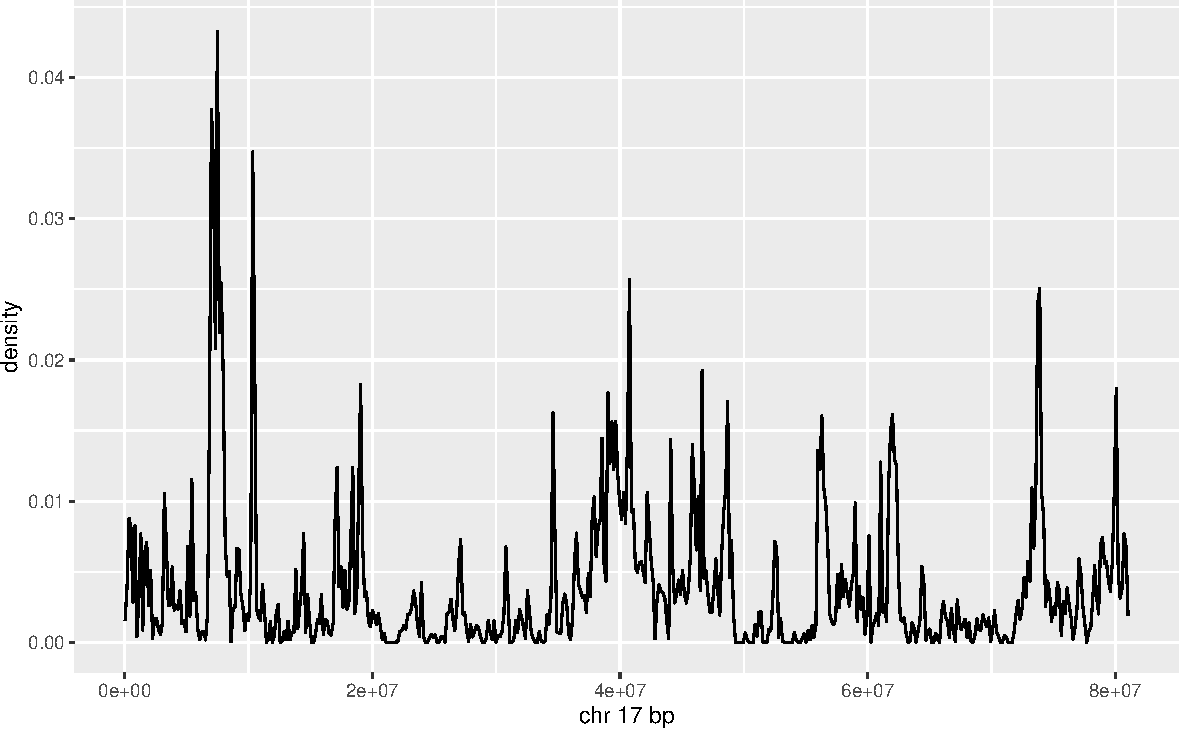
\includegraphics[width=1\linewidth,]{bioccb_files/figure-latex/mkden-1} \caption{Density of recurrent genomic alterations on chromosome 17 for 48 angiosarcoma patients.}\label{fig:mkden}
\end{figure}



\section{Genomic annotation resources relevant to cancer}\label{hubs}


\subsection{Resources from UCSC, NCBI, and EMBL}\label{resources-from-ucsc-ncbi-and-embl}

Sequences for reference genome builds for human and
other model organisms are supplied in BSgenome packages.
BSgenome.Hsapiens.UCSC.hg19 provides all chromosomes and
contigs for the 2009 build; the hg38 suffix may be used
for the 2013 build. The recent ``telomere to telomere''
build is available as BSgenome.Hsapiens.NCBI.T2T.CHMv13v2.0.

NCBI's dbSNP catalog of genetic variants is provided
in versioned packages.
For example, SNPlocs.Hsapiens.dbSNP155.GRCh38 includes
position and nucleotide content information for over
1 billion SNP identifiers ("rs numbers").

Tracks defined for the UCSC genome browser are also
packaged. The package 
\begin{verbatim}
TxDb.Hsapiens.UCSC.knownGene.hg38 
\end{verbatim} 
can be
used to get gene, transcript, and exon location information
for the hg38 build. The EnsDb packages provide similar
information for annotations curated at EMBL.

%\begin{shaded}
%\KeywordTok{library}\NormalTok{(EnsDb.Hsapiens.v86)}
%\NormalTok{EnsDb.Hsapiens.v86}
%\CommentTok{\#\# EnsDb for Ensembl:}
%\CommentTok{\#\# |Backend: SQLite}
%\CommentTok{\#\# |Db type: EnsDb}
%\CommentTok{\#\# |Type of Gene ID: Ensembl Gene ID}
%\CommentTok{\#\# |Supporting package: ensembldb}
%\CommentTok{\#\# |Db created by: ensembldb package from Bioconductor}
%\CommentTok{\#\# |script\_version: 0.3.0}
%\CommentTok{\#\# |Creation time: Thu May 18 16:32:27 2017}
%\CommentTok{\#\# |ensembl\_version: 86}
%\CommentTok{\#\# |ensembl\_host: localhost}
%\CommentTok{\#\# |Organism: homo\_sapiens}
%\CommentTok{\#\# |taxonomy\_id: 9606}
%\CommentTok{\#\# |genome\_build: GRCh38}
%\CommentTok{\#\# |DBSCHEMAVERSION: 2.0}
%\CommentTok{\#\# | No. of genes: 63970.}
%\CommentTok{\#\# | No. of transcripts: 216741.}
%\CommentTok{\#\# |Protein data available.}
%\end{Highlighting}
%\end{shaded}

\begin{shaded}
\begin{verbatim}
library(EnsDb.Hsapiens.v86)
EnsDb.Hsapiens.v86
## EnsDb for Ensembl:
## |Backend: SQLite
## |Db type: EnsDb
## |Type of Gene ID: Ensembl Gene ID
## |Supporting package: ensembldb
## |Db created by: ensembldb package from Bioconductor
## |script\_version: 0.3.0
## |Creation time: Thu May 18 16:32:27 2017
## |ensembl\_version: 86
## |ensembl\_host: localhost
## |Organism: homo\_sapiens
## |taxonomy\_id: 9606
## |genome\_build: GRCh38
## |DBSCHEMAVERSION: 2.0
## | No. of genes: 63970.
## | No. of transcripts: 216741.
## |Protein data available.
\end{verbatim}
\end{shaded}


The ``genes'' method provides addresses and additional
annotations.

\begin{shaded}
\begin{verbatim}
names(mcols(genes(EnsDb.Hsapiens.v86)))
## [1] "gene_id"          "gene_name"        "gene_biotype"     
## [4] "seq_coord_system" "symbol"           "entrezid"
head(table(genes(EnsDb.Hsapiens.v86)$gene_biotype))
##      3prime_overlapping_ncRNA                     antisense 
##                            30                          5703 
## bidirectional_promoter_lncRNA                     IG_C_gene 
##                             4                            23 
##               IG_C_pseudogene                     IG_D_gene 
##                            11                            64
\end{verbatim}
\end{shaded}

More recent versions of Ensembl gene annotation are available
from AnnotationHub, as illustrated above in section \ref{cache} with
the creation of \texttt{ens110}.

\subsection{Gene sets}\label{gene-sets}

Many methods have been developed to employ collections
of genes for inference on hypotheses about cancer
initiation or progression. The Molecular Signatures Database (MSigDB)
is curated at Broad Institute, and can be harvested
using the msigdb package.

Collect all gene sets for humans:

\begin{shaded}
\begin{verbatim}
library(msigdb)
hssigs = getMsigdb(org="hs", id="SYM", version=getMsigdbVersions())
\end{verbatim}
\end{shaded}

Find those with CANCER in their name:

\begin{shaded}
\begin{verbatim}
nms = grep("CANCER", names(hssigs), value=TRUE)
head(nms)
## [1] "SOGA_COLORECTAL_CANCER_MYC_DN"
## [2] "SOGA_COLORECTAL_CANCER_MYC_UP"
## [3] "WATANABE_RECTAL_CANCER_RADIOTHERAPY_RESPONSIVE_UP"
## [4] "LIU_PROSTATE_CANCER_UP"
## [5] "BERTUCCI_MEDULLARY_VS_DUCTAL_BREAST_CANCER_UP"
## [6] "WATANABE_COLON_CANCER_MSI_VS_MSS_UP"
wangmet = hssigs[["WANG_METASTASIS_OF_BREAST_CANCER_ESR1_UP"]]
wangmet
## setName: WANG_METASTASIS_OF_BREAST_CANCER_ESR1_UP
## geneIds: KPNA2, HDGFL3, ..., PSMC2 (total: 22)
## geneIdType: Symbol
## collectionType: Broad
##bcCategory: c2 (Curated)
##bcSubCategory: CGP
## details: use 'details(object)'
\end{verbatim}
\end{shaded}

Information on provenance is bound together with the gene list:

\begin{shaded}
\begin{verbatim}
details(wangmet)
## setName: WANG_METASTASIS_OF_BREAST_CANCER_ESR1_UP
## geneIds: KPNA2, HDGFL3, ..., PSMC2 (total: 22)
## geneIdType: Symbol
## collectionType: Broad
##bcCategory: c2 (Curated)
##bcSubCategory: CGP
## setIdentifier: LVY1HGGWMJ7:35020:Fri May 26 13:33:02 2023:1104005
## description: Genes whose expression in primary ER(+) 
##      [GeneID=2099] breast cancer tumors positively correla
## (longDescription available)
## organism: Homo sapiens
## pubMedIds: 15721472
## urls: https://data.broadinstitute.org/gsea-msigdb/msigdb/
##    release/2023.1.Hs/msigdb_v2023.1.Hs.xml.zip
## contributor: Arthur Liberzon
\end{verbatim}
\end{shaded}

\subsection{Ontologies}\label{ontologies}

Informal reasoning about cancer genomics employs conventional
but frequently ambiguous terminology. In modern
information science, ontologies are structured vocabularies
(sets of ``terms'', which may be single words or natural language
phrases) accompanied by
explicit statements of semantic relationships among terms.

Bioconductor provides several approaches for using ontologies
in cancer data science. The most familiar ontology
in this domain is Gene Ontology (GO), which organizes vocabulary
about genes and gene products in
the areas of molecular function, cellular components, and
biological processes.

\subsubsection{Ontology usage with AnnotationDbi}\label{ontology-usage-with-annotationdbi}

A common use case is to find genes or proteins associated
with some biological process, component, or function.
A phrase like `Golgi membrane' can be found in Gene Ontology
using the select method with GO.db:

\begin{shaded}
\begin{verbatim}
library(GO.db)
select(GO.db, keytype="TERM",
keys="Golgi membrane", columns=c("GOID", "DEFINITION", "ONTOLOGY"))
##             TERM       GOID
## 1 Golgi membrane GO:0000139
##                                 DEFINITION
## 1 The lipid bilayer surrounding any of the 
## compartments of the Golgi apparatus.
## ONTOLOGY
## 1     CC
\end{verbatim}
\end{shaded}

Once the formal identifier is obtained, the org.Hs.eg.db package can be used to find mappings
from the GO term to gene and protein identifiers. This generates a fairly large table:

\begin{shaded}
\begin{verbatim}
library(org.Hs.eg.db)
go139 = select(org.Hs.eg.db, keys="GO:0000139", keytype="GO",
columns=c("ENTREZID", "SYMBOL", "PFAM"))
dim(go139)
## [1] 1212 6
head(go139)
##           GO EVIDENCE ONTOLOGY ENTREZID SYMBOL    PFAM
## 1 GO:0000139      TAS       CC       28    ABO PF03414
## 2 GO:0000139      IEA       CC      102 ADAM10 PF00200
## 3 GO:0000139      IEA       CC      102 ADAM10 PF13574
## 4 GO:0000139      IEA       CC      102 ADAM10 PF01562
## 5 GO:0000139      TAS       CC      162  AP1B1 PF09066
## 6 GO:0000139      TAS       CC      162  AP1B1 PF01602
\end{verbatim}
\end{shaded}

The evidence code TAS means that there is a ``traceable author statement'' associating the term
of interest with the gene identified. The number of genes in traceable Golgi membrane:gene
associations is found with

\begin{shaded}
\begin{verbatim}
go139 |> dplyr::filter(EVIDENCE=="TAS") |> distinct(ENTREZID) |> count()
##       n
## [1] 327
\end{verbatim}
\end{shaded}


\subsubsection{Ontology usage with rols}\label{ontology-usage-with-rols}

Access to a vast collection of ontologies is afforded by the EBI's
Ontology Lookup Service (OLS). The rols package uses the OLS API
to discover ontologic mapping of terms of interest. Here we'll
consider the term ``golgi membrane dynamics'', which is not found in GO.
Again a multistep process is used.

\begin{shaded}
\begin{verbatim}
library(rols)
lk1 = OlsSearch(q="golgi membrane dynamics", exact=TRUE)
lk1
## Object of class 'OlsSearch':
##query: golgi membrane dynamics
##requested: 20 (out of 3)
##response(s): 0
\end{verbatim}
\end{shaded}


In this first step, we find how extensive is the response
to the query. Certain searches yield tens of thousands of hits.
With the exact parameter setting, the yield is modest.
Now we extract a data.frame after requesting all
records with \texttt{olsSearch}.  Results are
excerpted in Table \ref{tab:tab-golg}.

\begin{shaded}
\begin{verbatim}
lk2 = olsSearch(lk1)
lk3 = as(lk2, "data.frame")
lk3$description = unlist(lk3$description)
\end{verbatim}
\end{shaded}



\begin{table}
\caption{Using rols to obtain ontologic information related to
golgi membrane dynamics. \label{tab:tab-golg}}
\begin{tabular}{lp{5cm}p{8cm}}
\toprule
short\_form & description & label\\
\midrule
NCIT\_C119637 & This gene is involved in both protein ubiquitination and Golgi membrane dynamics. & HACE1 Gene\\
NCIT\_C119639 & E3 ubiquitin-protein ligase HACE1 (909 aa, \textasciitilde{}102 kDa) is encoded by the human HACE1 gene. This protein is involved in the regulation of both the ubiquitination and subsequent degradation of small GTPases, which modulates Golgi membrane dynamics. & E3 Ubiquitin-Protein Ligase HACE1\\
NCIT\_C119638 & Human HACE1 wild-type allele is located in the vicinity of 6q16.3 and is approximately 132 kb in length. This allele, which encodes E3 ubiquitin-protein ligase HACE1 protein, plays a role in the modulation of both Golgi membrane dynamics and ubiquitination. Mutations of the gene, including translocations that either reduce expression of the gene (t(6;15)(q21;q21)) or truncate the gene (t(5;6)(q21;q21)), are associated with Wilms tumor. & HACE1 wt Allele\\
\bottomrule
\end{tabular}
\end{table}

The detailed descriptions of the NCI Thesaurus entries show
the exact nature of the search outcome.

\subsubsection{Cross-ontology relationships}\label{cross-ontology-relationships}

Philosophically, ontology is the study of what there is. For
applications in information
science,
boundaries need to be established so that ontological
resources can be managed with well-defined scopes. In Gene
Ontology, three sub-ontologies are explicitly identified for
cellular components, biological processes, and molecular functions.

As knowledge of cell biology increases, the typology of
cells becomes more and more intricate. Differentiation
and definition
of ``cell types'' involves concepts from immunology,
protein science, anatomy, and other conceptual domains
for which ontologies have been developed. Figure \ref{fig:ontopair}
presents, on the left, the hierarchy of cell type concepts starting at ``lymphocyte'',
leading to ``Type II Natural Killer T cell secreting interferon gamma''.
On the right, some of the GO and Protein Ontology (PR) cross-references
in the Cell Ontology (CL) entry for the Type II NK cell are shown.
The ``cond'' column of the table contains abbreviated tokens
representing formal relationships linking the cell type
to the protein or cellular component elements of PR and GO.
The token ``hasPMP'' refers to the element of the Relation Ontology
(RO) ``has plasma membrane part'' (RO:0002104).

\begin{figure}
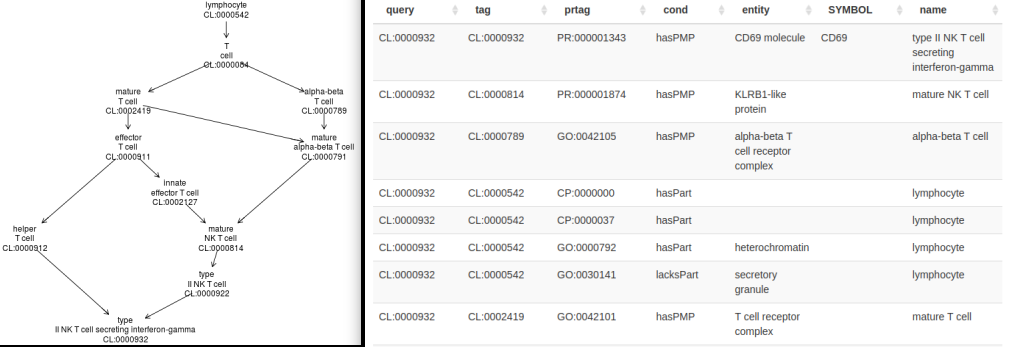
\includegraphics[width=1\linewidth,]{ontoPair} \caption{Ontology visualization and tabulation with ontoProc::ctmarks.}\label{fig:ontopair}
\end{figure}

Prospects for use of ontological discipline in the
definition of new cell types are reviewed in a 2018
paper from the Venter Institute \cite{Aevermann2018}.

The field of biological ontology is rapidly advancing,
and the integration of ontology search and inference
with data analytic frameworks requires more effort at this time.




\section{Analytical workflows}\label{analytical-workflows}


\subsection{Overview}\label{overview}

Table \ref{tab:tab-wflow} presents an informal topical
labeling for Bioconductor software packages with
cancer mentioned in the Description field of package
metadata.

\begin{table}
\caption{\label{tab:tab-wflow}Topical organization of packages with cancer applications.}
\begin{tabular}{l{4cm}p{6cm}}
\toprule
topic & packages\\
\midrule
Ancestry & RAIDS\\
Biomarkers & INDEED, iPath, RLassoCox\\
ceRNA & GDCRNATools\\
Clonal Evolution & CIMICE, LACE, OncoSimulR, TRONCO, CancerInSilico, cellscape\\
CNV & oncoscanR, SCOPE, ZygosityPredictor\\
\addlinespace
DrugSensitivity & DepInfeR, octad, PharmacoGx, rcellminer\\
Epigenetics & MethylMix, AMARETTO, COCOA, methylclock, missMethyl\\
HotSpots/Drivers/signatures & compSPOT, MoonlightR, Moonlight2R, \\
 & DriverNet, genefu, mastR, pathifier, RESOLVE, macat, \\
 & SigCheck, signeR, signifinder, supersigs, decompTumor2Sig, YAPSA\\
ImmuneModulation & easier\\
IsoformSwitching & IsoformSwitchAnalyzeR\\
\addlinespace
Literature mining & OncoScore\\
ncRNA & NoRCE\\
Radiomics & RadioGx\\
RecurrentFusion & copa, oppar\\
Spatial & SpatialDecon\\
\addlinespace
SpecificCancers & consensusOV, PDATK, STROMA4\\
Splicing & OutSplice, psichomics\\
Subtyping & SCFA\\
\end{tabular}
\bottomrule
\end{table}

The vignettes of each of these packages provide background and
illustration of their roles in cancer genomics.

\subsection{Packages supporting epigenomic analysis}\label{packages-supporting-epigenomic-analysis}

Bioconductor also provides a diverse array of packages for analysis of epigenome
data. Cancer is often studied under a developmental lens, so increasingly, studies
are measuring cell states using epigenomic methods. Epigenomics is the study of
chemical modifications and chromosomal conformations of DNA in a nucleus; in cancer
epigenomics, we study how the cancer epigenome differs among cancers and how
these relate to healthy epigenomes. As of 2023, Bioconductor includes 89 packages
under \emph{Epigenetics} and 93 packages tagged under \emph{FunctionalGenomics}, including dozens of tools
for analyzing a variety of epigenome assays, such as ATAC-seq, ChIP-seq, or
bisulfite-seq. Among these are also tools that handle more general analysis, such
as genomic region set enrichment.

First, for ATAC-seq data, bioconductor packages include general-purpose pipelines, including scPipe
\cite{Tian2018}. %(Tian et al. \protect\hyperlink{ref-Tian2018}{2018})
and esATAC \cite{Wei2018} %(Wei et al. \protect\hyperlink{ref-Wei2018}{2018}), 
which start from FASTQ files and produce feature count
matrices. Alternatively, many practitioners elect to do general-purpose pipeline processing outside of
R, and then bring the processed data into R for statistical analysis,
visualization, and quality control. In this approach, ATACseqQC
provides
a variety of QC plots specific to ATAC-seq data \cite{Ou2018}.% (Ou et al. \protect\hyperlink{ref-Ou2018}{2018}).

For DNA methylation, many popular packages have been developed to help with
all stages of a DNA methylation analysis. These include minfi 
\cite{Aryee2014}
which specializes in methylation array analysis, biseq and bsseq \cite{Hansen2012}  %(Hansen, Irizarry, and Wu \protect\hyperlink{ref-Hansen2012}{2012})
which provide fundamental infrastructure for sequencing-based assays, and RnBeads
\cite{Mueller2019},
%(Müller et al. \protect\hyperlink{ref-Mueller2019}{2019}), 
which provides a comprehensive general-purpose analysis of DNA
methylation cohorts from arrays or sequencing-based assays. Other packages provide more specialized
analysis approaches, such as MIRA \cite{Lawson2018}, %(Lawson et al. \protect\hyperlink{ref-Lawson2018}{2018}), 
which infers regulatory
activity of transcription factors using DNA methylation signals, %(Sheffield et al.~2018), FIXME not found
or ELMER, which uses DNA methylation and gene expression in large cancer
cohorts to infer transcription factor networks \cite{Silva2019}. % (Silva et al. \protect\hyperlink{ref-Silva2019}{2018}). 
EpiDISH infers
the proportions of cell-types present in a bulk sample on the basis
of DNA methylation data \cite{Zheng2018a}. %(Zheng et al. \protect\hyperlink{ref-Zheng2018a}{2018}).

%Another popular epigenome experiment is ChIP-seq, and Bioconductor delivers many packages in
%this area. 
DiffBind \cite{Stark2011} %(Stark and Brown \protect\hyperlink{ref-Stark2011}{2011}) is a popular approach for
facilitates differential binding analysis of ChIP-seq peak data.

%A variety of packages are also geared toward visualization of this type
%of data. 
GenomicDistributions \cite{Kupkova2022} % (Kupkova et al. \protect\hyperlink{ref-Kupkova2022}{2022}) 
provides a variety of plots for visualization
distributions of any type of genomic range data. The chromPlot package specializes
in plots across chromosomes.  Several packages deal with
unsupervised exploration of variation in epigenomic data. PathwayPCA, MOFA2 \cite{Argelaguet2020} %(Argelaguet et al. \protect\hyperlink{ref-Argelaguet2020}{2020})
and COCOA \cite{Lawson2020} %(Lawson et al. \protect\hyperlink{ref-Lawson2020}{2020}) 
can process any epigenomic signal data.
A variety of alternative approaches for enrichment analysis, which include LOLA \cite{Sheffield2016}, %(Sheffield and Bock \protect\hyperlink{ref-Sheffield2016}{2016}),
chipenrich, regionR \cite{Gel2015}, %(Gel et al. \protect\hyperlink{ref-Gel2015}{2015}), 
and FGNet \cite{Aibar2015}. %(Aibar et al. \protect\hyperlink{ref-Aibar2015}{2015}).
Annotation packages include ChIPpeakAnno \cite{Zhu2010} % (Zhu et al. \protect\hyperlink{ref-Zhu2010}{2010})
and annotatr \cite{Cavalcante2017}.%(Cavalcante and Sartor \protect\hyperlink{ref-Cavalcante2017}{2017}) are popular packages for annotating genomic
%ranges.


\subsection{Some details on prediction of responsiveness to immune checkpoint blockade}\label{some-details-on-prediction-of-responsiveness-to-immune-checkpoint-blockade}

The National Cancer Institute website on checkpoint inhibitors
in cancer immunotherapy (``Immune Checkpoint Inhibitors'' 
\cite{ICBnci}) %\protect\hyperlink{ref-ICBnci}{2022})
lists 12 different cancer types
amenable to treatment via immune checkpoint inhibition.
The ``easier'' package in Bioconductor
assembles multiple systems biology resources
to produce patient-specific
prediction of responsiveness to
immune checkpoint blockade (ICB) \cite{easierPap}. %, as described in Lapuente-Santana et al. (\protect\hyperlink{ref-easierPap}{2021}).

Figure \ref{fig:easfin} presents on overview of results of
immune response assessment in a cohort of patients with
bladder cancer \cite{Mariathasan2018}. %reported in Mariathasan et al. (\protect\hyperlink{ref-Mariathasan2018}{2018}).
Patient's bulk RNA-seq data are used to develop multiple
quantitative descriptors of the tumor microenvironment,
and scores for processes regarded as hallmarks of anti-cancer
immune responses.

\begin{figure}
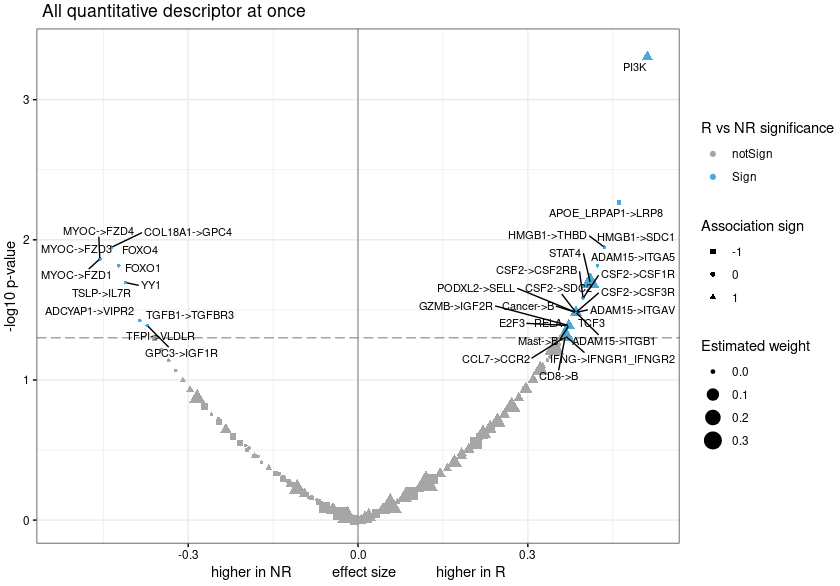
\includegraphics[width=0.95\linewidth,]{easierFinal} \caption{Comparison of genomic features distinguishing patients non-responsive and responsive to immune checkpoint blockade.}\label{fig:easfin}
\end{figure}

This display encapsulates a) the capacity of measurements of
genomic elements to discriminate patients who respond
to ICB for bladder cancer (position of labeled
item on x axis), b) the direction of association of
element activity with immune response (shape of glyph) and c) the
relative magnitudes of weights (size of glyph) estimated for features in
initial model fitting.

The design of this package is noteworthy in its approach
to information hiding. Parameters estimated in machine
learning of tissue-specific relations between quantitative
descriptors of the tumor microenvironment and hallmarks
of immune response are stored in ExperimentHub.

\begin{shaded}
\begin{verbatim}
library(easierData)
list_easierData()
##   eh_id                            title
##  EH6677   Mariathasan2018_PDL1_treatment
##  EH6678                       opt_models
##  EH6679                 opt_xtrain_stats
##  EH6680              TCGA_mean_pancancer
##  EH6681                TCGA_sd_pancancer
##  EH6682                 cor_scores_genes
##  EH6683               intercell networks
##  EH6684                lr_frequency_TCGA
##  EH6685                   group_lr_pairs
##  EH6686                  HGNC_annotation
##  EH6687           scores_signature_genes
\end{verbatim}
\end{shaded}

The structure of the stored model weights resource can be sketched by probing list elements.

\begin{shaded}
\begin{verbatim}
mw = eh[["EH6678"]]
## see ?easierData and browseVignettes('easierData') for documentation
## loading from cache
names(mw)   # TCGA tumor types
##  [1] "LUAD" "LUSC" "BLCA" "BRCA" "CESC" "CRC"  "GBM"  "HNSC" "KIRC"
## [10] "KIRP" "LIHC"   "OV" "PAAD" "PRAD" "SKCM" "STAD" "THCA" "UCEC"
## [19] "NSCLC"
names(mw[["LUAD"]]) # TME descriptors
## [1] "pathways" "immunecells" "tfs" "lrpairs" "ccpairs"
rownames(mw[["LUAD"]]$pathways$CYT) # predict cytolytic activity
##  [1] "(Intercept)" "Androgen" "EGFR" "Estrogen" "Hypoxia"
##  [6]    "JAK-STAT"     "MAPK" "NFkB" "p53"      "PI3K"
## [11]        "TNFa"    "Trail" "VEGF" "WNT"
\end{verbatim}
\end{shaded}


The vignette of the easier package steps through phases,
using these tumor-type-specific weights to compute patient-specific measures
of transcription factor activity or cell-cell interaction on the basis of bulk
RNA-seq (units are transcripts per million), and a patient-specific
measure of pathway activity using raw RNA-seq counts. These metrics
may be of interest in their own right for applications other than
establishing predictions of response to ICB.

Section \ref{app3} provides the names and versions of all packages
used to produce this analysis.



%\begin{thebibliography}{99.}%

\bibitem{ref-Aevermann2018}
Aevermann, Brian D., Mark Novotny, Trygve Bakken, Jeremy A. Miller, Alexander D. Diehl, David Osumi-Sutherland, Roger S. Lasken, Ed S. Lein, and Richard H. Scheuermann. 2018. ``Cell Type Discovery Using Single-Cell Transcriptomics: Implications for Ontological Representation.'' \emph{Human Molecular Genetics} 27 (R1): R40--R47. \url{https://doi.org/10.1093/hmg/ddy100}.

\bibitem{ref-Aganezov2022}
Aganezov, Sergey, Stephanie M. Yan, Daniela C. Soto, Melanie Kirsche, Samantha Zarate, Pavel Avdeyev, Dylan J. Taylor, et al. 2022. ``A Complete Reference Genome Improves Analysis of Human Genetic Variation.'' \emph{Science} 376 (6588). \url{https://doi.org/10.1126/science.abl3533}.

\bibitem{ref-Aibar2015}
Aibar, Sara, Celia Fontanillo, Conrad Droste, and Javier De Las Rivas. 2015. ``Functional Gene Networks: R/Bioc Package to Generate and Analyse Gene Networks Derived from Functional Enrichment and Clustering.'' \emph{Bioinformatics} 31 (10): 1686--8. \url{https://doi.org/10.1093/bioinformatics/btu864}.

\bibitem{ref-Argelaguet2020}
Argelaguet, Ricard, Damien Arnol, Danila Bredikhin, Yonatan Deloro, Britta Velten, John C. Marioni, and Oliver Stegle. 2020. ``MOFA+: A Statistical Framework for Comprehensive Integration of Multi-Modal Single-Cell Data.'' \emph{Genome Biology} 21 (1). \url{https://doi.org/10.1186/s13059-020-02015-1}.

\bibitem{ref-Aryee2014}
Aryee, Martin J., Andrew E. Jaffe, Hector Corrada-Bravo, Christine Ladd-Acosta, Andrew P. Feinberg, Kasper D. Hansen, and Rafael A. Irizarry. 2014. ``Minfi: A Flexible and Comprehensive Bioconductor Package for the Analysis of Infinium Dna Methylation Microarrays.'' \emph{Bioinformatics} 30 (10): 1363--9. \url{https://doi.org/10.1093/bioinformatics/btu049}.

\bibitem{ref-Cavalcante2017}
Cavalcante, Raymond G, and Maureen A Sartor. 2017. ``Annotatr: Genomic Regions in Context.'' Edited by Alfonso Valencia. \emph{Bioinformatics} 33 (15): 2381--3. \url{https://doi.org/10.1093/bioinformatics/btx183}.

\bibitem{ref-Couto2023}
Couto, Bárbara Zita Peters, Nicholas Robertson, Ellis Patrick, and Shila Ghazanfar. 2023. ``MoleculeExperiment Enables Consistent Infrastructure for Molecule-Resolved Spatial Transcriptomics Data in Bioconductor.'' \emph{bioRxiv}. \url{https://doi.org/10.1101/2023.05.16.541040}.

\bibitem{ref-Gel2015}
Gel, Bernat, Anna Diez-Villanueva, Eduard Serra, Marcus Buschbeck, Miguel A. Peinado, and Roberto Malinverni. 2015. ``regioneR: An R/Bioconductor Package for the Association Analysis of Genomic Regions Based on Permutation Tests.'' \emph{Bioinformatics}, September, btv562. \url{https://doi.org/10.1093/bioinformatics/btv562}.

\bibitem{ref-Hansen2012}
Hansen, Kasper D., Rafael a. Irizarry, and Zhijin Wu. 2012. ``Removing Technical Variability in Rna-Seq Data Using Conditional Quantile Normalization.'' \emph{Biostatistics} 13: 204--16. \url{https://doi.org/10.1093/biostatistics/kxr054}.

\bibitem{ref-ICBnci}
``Immune Checkpoint Inhibitors.'' 2022. \url{https://www.cancer.gov/about-cancer/treatment/types/immunotherapy/checkpoint-inhibitors}.

\bibitem{ref-Kupkova2022}
Kupkova, Kristyna, Jose Verdezoto Mosquera, Jason P. Smith, Michał Stolarczyk, Tessa L. Danehy, John T. Lawson, Bingjie Xue, John T. Stubbs, Nathan LeRoy, and Nathan C. Sheffield. 2022. ``GenomicDistributions: Fast Analysis of Genomic Intervals with Bioconductor.'' \emph{BMC Genomics} 23 (1). \url{https://doi.org/10.1186/s12864-022-08467-y}.

\bibitem{ref-easierPap}
Lapuente-Santana, Óscar, Maisa van Genderen, Peter A. J. Hilbers, Francesca Finotello, and Federica Eduati. 2021. ``Interpretable Systems Biomarkers Predict Response to Immune-Checkpoint Inhibitors.'' \emph{Patterns} 2 (8). \url{https://doi.org/10.1016/j.patter.2021.100293}.

\bibitem{ref-Lawson2018}
Lawson, John, Eleni Tomazou, Christoph Bock, and Nathan C. Sheffield. 2018. ``MIRA: An R Package for DNA Methylation-Based Inference of Regulatory Activity.'' \emph{Bioinformatics} bty083 (March). \url{https://doi.org/10.1093/bioinformatics/bty083}.

\bibitem{ref-Lawson2020}
Lawson, John T., Jason P. Smith, Stefan Bekiranov, Francine E. Garrett-Bakelman, and Nathan C. Sheffield. 2020. ``COCOA: Coordinate Covariation Analysis of Epigenetic Heterogeneity.'' \emph{Genome Biology} 21 (1). \url{https://doi.org/10.1186/s13059-020-02139-4}.

\bibitem{ref-Mariathasan2018}
Mariathasan, Sanjeev, Shannon J. Turley, Dorothee Nickles, Alessandra Castiglioni, Kobe Yuen, Yulei Wang, Edward E. Kadel III, et al. 2018. ``TGFB Attenuates Tumour Response to Pd-L1 Blockade by Contributing to Exclusion of T Cells.'' \emph{Nature} 554 (7693): 544--48. \url{https://doi.org/10.1038/nature25501}.

\bibitem{ref-moses23}
Moses, Lambda, Pétur Helgi Einarsson, Kayla Jackson, Laura Luebbert, A Sina Booeshaghi, Sindri Antonsson, Nicolas Bray, Páll Melsted, and Lior Pachter. 2023. ``Voyager: Exploratory Single-Cell Genomics Data Analysis with Geospatial Statistics.'' \emph{bioRxiv}.

\bibitem{ref-Mueller2019}
Müller, Fabian, Michael Scherer, Yassen Assenov, Pavlo Lutsik, Jörn Walter, Thomas Lengauer, and Christoph Bock. 2019. ``RnBeads 2.0: Comprehensive Analysis of Dna Methylation Data.'' \emph{Genome Biology} 20 (1). \url{https://doi.org/10.1186/s13059-019-1664-9}.

\bibitem{ref-Ou2018}
Ou, Jianhong, Haibo Liu, Jun Yu, Michelle A. Kelliher, Lucio H. Castilla, Nathan D. Lawson, and Lihua Julie Zhu. 2018. ``ATACseqQC: A Bioconductor Package for Post-Alignment Quality Assessment of Atac-Seq Data.'' \emph{BMC Genomics} 19 (1). \url{https://doi.org/10.1186/s12864-018-4559-3}.

\bibitem{ref-rig22}
Righelli, Dario, Lukas M Weber, Helena L Crowell, Brenda Pardo, Leonardo Collado-Torres, Shila Ghazanfar, Aaron TL Lun, Stephanie C Hicks, and Davide Risso. 2022. ``SpatialExperiment: Infrastructure for Spatially-Resolved Transcriptomics Data in R Using Bioconductor.'' \emph{Bioinformatics} 38 (11): 3128--31.

\bibitem{ref-Schatz2022}
Schatz, Michael C., Anthony A. Philippakis, Enis Afgan, Eric Banks, Vincent J. Carey, Robert J. Carroll, Alessandro Culotti, et al. 2022. ``Inverting the Model of Genomics Data Sharing with the Nhgri Genomic Data Science Analysis, Visualization, and Informatics Lab-Space.'' \emph{Cell Genomics} 2 (1): 100085. \url{https://doi.org/10.1016/j.xgen.2021.100085}.

\bibitem{ref-Sheffield2016}
Sheffield, Nathan C., and Christoph Bock. 2016. ``LOLA: Enrichment Analysis for Genomic Region Sets and Regulatory Elements in R and Bioconductor.'' \emph{Bioinformatics} 32 (4): 587--89. \url{https://doi.org/10.1093/bioinformatics/btv612}.

\bibitem{ref-Silva2019}
Silva, Tiago C., Simon G. Coetzee, Nicole Gull, Lijing Yao, Dennis J. Hazelett, Houtan Noushmehr, De-Chen Lin, and Benjamin P. Berman. 2018. ``ELMER V.2: An R/Bioconductor Package to Reconstruct Gene Regulatory Networks from Dna Methylation and Transcriptome Profiles.'' Edited by Oliver Stegle. \emph{Bioinformatics} 35 (11): 1974--7. \url{https://doi.org/10.1093/bioinformatics/bty902}.

\bibitem{ref-Stark2011}
Stark, Rory, and Gordon Brown. 2011. ``DiffBind: Differential Binding Analysis of Chip-Seq Peak Data.''

\bibitem{ref-Tian2018}
Tian, Luyi, Shian Su, Xueyi Dong, Daniela Amann-Zalcenstein, Christine Biben, Azadeh Seidi, Douglas J. Hilton, Shalin H. Naik, and Matthew E. Ritchie. 2018. ``ScPipe: A Flexible R/Bioconductor Preprocessing Pipeline for Single-Cell Rna-Sequencing Data.'' Edited by Mihaela Pertea. \emph{PLOS Computational Biology} 14 (8): e1006361. \url{https://doi.org/10.1371/journal.pcbi.1006361}.

\bibitem{ref-webr23}
Weber, Lukas M, Arkajyoti Saha, Abhirup Datta, Kasper D Hansen, and Stephanie C Hicks. 2023. ``NnSVG for the Scalable Identification of Spatially Variable Genes Using Nearest-Neighbor Gaussian Processes.'' \emph{Nature Communications} 14 (1): 4059.

\bibitem{ref-Wei2018}
Wei, Zheng, Wei Zhang, Huan Fang, Yanda Li, and Xiaowo Wang. 2018. ``EsATAC: An Easy-to-Use Systematic Pipeline for Atac-Seq Data Analysis.'' \emph{Bioinformatics (Oxford, England)}, March. \url{https://doi.org/10.1093/bioinformatics/bty141}.

\bibitem{ref-Zheng2018a}
Zheng, Shijie C., Charles E. Breeze, Stephan Beck, and Andrew E. Teschendorff. 2018. ``Identification of Differentially Methylated Cell Types in Epigenome-Wide Association Studies.'' \emph{Nature Methods} 15 (12): 1059--66. \url{https://doi.org/10.1038/s41592-018-0213-x}.

\bibitem{ref-Zhu2010}
Zhu, Lihua J, Claude Gazin, Nathan D Lawson, Hervé Pagès, Simon M Lin, David S Lapointe, and Michael R Green. 2010. ``ChIPpeakAnno: A Bioconductor Package to Annotate ChIP-Seq and ChIP-Chip Data.'' \emph{BMC Bioinformatics} 11 (1). \url{https://doi.org/10.1186/1471-2105-11-237}.

\end{thebibliography}

\bibliographystyle{authordate1}
\bibliography{biocmimb}

\end{document}
